\section{Experiments}
We evaluate the proposed algorithms on the following scenario: a collection of 3d-points $P = \{ p_1,\dots,p_s \} \subseteq \R^3$ is sampled from a number of $t$ planes which contain the coordinate origin. We wish to partition the resulting point cloud in such a way that makes the underlying set of planes obvious: i.e., all points that were sampled from a given plane are part of the same partition, distinct from the partitions of the other planes. The points are generated as follows:
\begin{enumerate}
    \item Every plane is defined by a normal vector and an orientation, i.e. we have vectors $\vec{n}_1,\dots,\vec{n}_t \in \R^3$ and orientations $\vec{o}_1,\dots,\vec{o}_t \in \R^3$. For each plane, we draw $\lambda_i,\lambda_i'$ from $\mathcal{U}([-\pi,\pi))$, and $x_i,x_i'$ from $\mathcal{U}([0,1))$ and determine $\varphi_i = \arccos(2x_i-1), \varphi_i' = \arccos(2x_i'-1)$\footnote{Source: Jason Davies, \href{https://www.jasondavies.com/maps/random-points/}{https://www.jasondavies.com/maps/random-points/}. Accessed on 6th December 2020.}. The vectors are computed by $$ \vec{n}_i = \begin{bmatrix} \sin(\varphi_i) \cos(\lambda_i) \\ \sin(\varphi_i)\sin(\lambda_i) \\ \cos(\varphi_i) \end{bmatrix},\quad \vec{h}_i = \begin{bmatrix} \sin(\varphi_i') \cos(\lambda_i') \\ \sin(\varphi_i')\sin(\lambda_i') \\ \cos(\varphi_i') \end{bmatrix} \times \vec{n}_i,\quad \vec{o}_i = \frac{\vec{h}_i}{||\vec{h}_i||} $$
    \item For every point $p_i$, three components are sampled: the 2d-position on the plane $x_i,y_i$ from $\mathcal{U}([-1,1])$, and a noise-component $z_i$ from $\mathcal{U}([-\epsilon,\epsilon])$ (where $\epsilon$ indicates the level of noise). The point is then transformed into plane-space, i.e. $$ p_i = x_i \vec{o}_i + y_i \vec{u}_i + z_i \vec{n}_i, $$ where $\vec{u}_i$ is the normalized cross-product between $\vec{n}_i$ and $\vec{o}_i$.
\end{enumerate}
For three points $u,v,w \in P$, we define the following cost-structure
\begin{align*}
    c(\{u,v,w\}) = 0,\quad c'(\{u,v,w\}) = \mathrm{d}(\{ u,v,w \},(0,0,0)) - \tau,
\end{align*}
where $\mathrm{d}(\{u,v,w\},p)$ is the distance between the plane that contains $u,v$ and $w$ and $p$ (``$\cdot$'' is the dot-product in this case):
\begin{align*}
    \mathrm{d}(\{u,v,w\},p) = \frac{\vec{n} \cdot (u - p)}{||\vec{n}||},\quad \vec{n} = (v-u)\times (w-u),
\end{align*}
and $\tau$ is some small value. Therefore, if the distance from the plane spanning over $u,v$ and $w$ to the origin ist smaller than $\tau$, it is considered ``good'' when $u,v$ and $w$ are part of the same partition and if the distance is large, it is considered ``bad''. As it turns out, these definitions of $c$ and $c'$ are sufficient to obtain the original partitions from unidentified point clouds.

\begin{figure}
    \centering
    \begin{subfigure}{.45\textwidth}
        \centering
        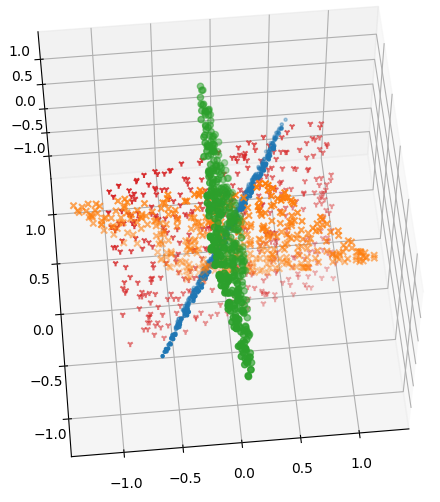
\includegraphics[width=\textwidth]{pics/points-400-400-400-400.png}
        \caption{Point cloud consisting of four planes with 400 points each and noise $\epsilon=0.01$.}
    \end{subfigure}%
    \hspace{2em}
    \begin{subfigure}{.45\textwidth}
        \centering
        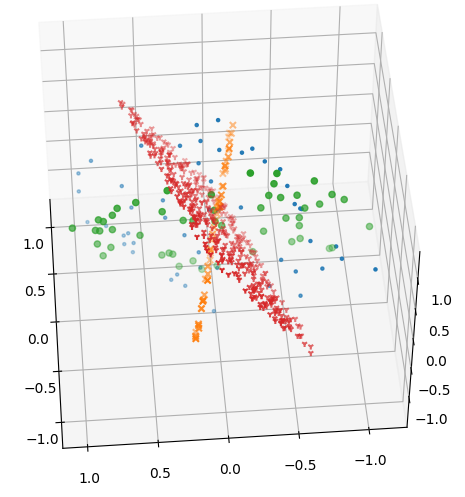
\includegraphics[width=\textwidth]{pics/points-50-50-50-400.png}
        \caption{Point cloud consisting of four planes, of which three have 50 points and one has 400 points with noise $\epsilon=0.01$.}
    \end{subfigure}
    \caption{Two possible point clouds.} \label{fig:point_cloud_examples}
\end{figure}